\documentclass[serif,mathserif,final]{beamer}
\mode<presentation>{\usetheme{Prisms}}
\usepackage{amsmath,amsfonts,amssymb,pxfonts,eulervm,xspace}
\usepackage{graphicx}
\usepackage{ragged2e}
\usepackage{psfrag}
\graphicspath{{./figures/}}
\usepackage[orientation=landscape,size=custom,width=119,height= 89, scale=1.16,debug]{beamerposter}

%-- Header and footer information ----------------------------------
\newcommand{\footleft}{\large {PRISMS: PRedictive Integrated Structural Materials Science\\ UM-DOE Software Innovation Center for Integrated Multi-Scale Modeling of Structural Metals}}
%\newcommand{\footright}{empty for now}
\title{Your Poster Title Goes Here}
\author{Author1$^1$ \quad Author2$^2$ \quad Author3$^1$ \quad Author4$^2$}
\institute{$^1$ Author Affiliation, City, Country \\ $^2$ Author Affiliation, City, Country}
%-------------------------------------------------------------------

%-- Main Document --------------------------------------------------
\begin{document}
\begin{frame}{}
  \begin{columns}[t]

    %-- Column 1 ---------------------------------------------------
    \begin{column}{0.32\linewidth}

      %-- Block 1-1
      \begin{block}{Goals}
        \justifying
        List your goals here. Can use text, itemize (bullet points), images, etc in this space.
         \vspace{2in}
        \begin{itemize}
        \item Goal 1
        \item Goal 2
        \item Goal 3
        \end{itemize}
        \vspace{2in}
        Or include equations:
        {\large
          \begin{align*}
            \nabla \cdot P  &= 0 \hspace{0.68\columnwidth} \text{\large \textit{sample equation}}
          \end{align*}
        }
        \vspace{5in}
      \end{block}
      \begin{figure}[htb]
        \centering
        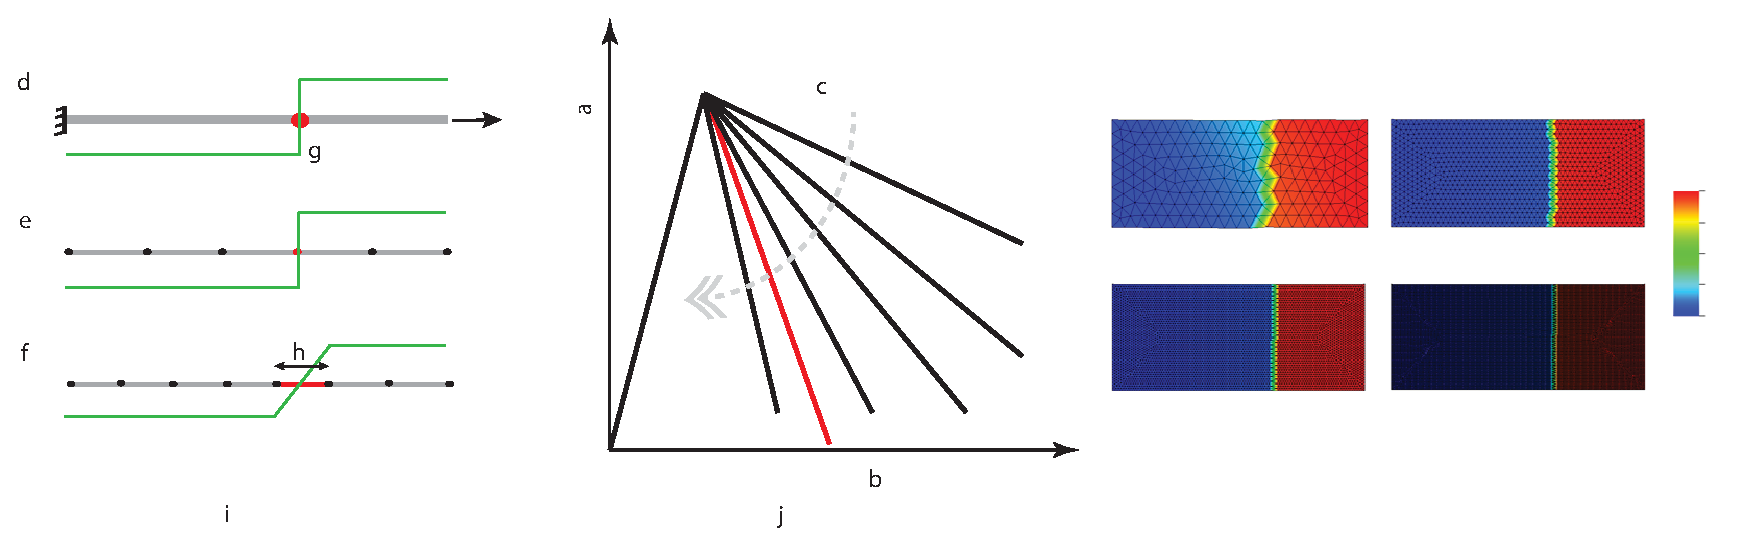
\includegraphics[width=0.85\columnwidth]{sampleFigure}
      \end{figure}
      \begin{center}
	{\large \textbf{Sample figure}}
      \end{center}
      
      %-- Block 1-2
      \begin{block}{Summary}
        \justifying
        Summary goes here. Can use text, itemize (bullet points), images, etc in this space.
        \begin{itemize}
        \item Summary 1
        \item Summary 2
        \end{itemize}
      \end{block}

    \end{column}%1

    %-- Column 2 ---------------------------------------------------
    \begin{column}{0.32\linewidth}

      %-- Block 2-1
      \begin{block}{Methodology}
        \justifying
        This is the main workspace and from here its upto the users discretion to plan the column layout, number of section, section titles, content, etc . 
        \vspace{5in}
      \end{block}
      
      %-- Block 2-2
      \begin{block}{Discussion}
        \vspace{5in}
      \end{block}

    %-- Block 2-3
    \begin{block}{Results}
       \vspace{5in}
     \end{block}
    \end{column}%2

    %-- Column 3 ---------------------------------------------------
    \begin{column}{0.32\linewidth}
      \vspace{1in}
      User can Continue the section from the previous column like this.
      \vspace{8in}

      %-- Block 3-1
      \begin{block}{Accomplishments}
        \justifying
         \vspace{2in}
        \begin{itemize}
        \item Accomplishment 1
        \item Accomplishment 2
        \item Accomplishment 3
        \end{itemize}
        \vspace{2in}
      \end{block}

      %\vskip2ex

      %-- Block 3-2
      \begin{block}{References}
        \justifying
            [1] Author 1 , Author 2, Author 3, ``Reference title''. \textit{Journal title}, Year.  
            \vskip1ex 
            [2] Author 1 , Author 2, Author 3, ``Reference title''. \textit{Journal title}, Year.  
      \end{block}

    \end{column}

  \end{columns}
\end{frame}
\end{document}
%http://www-personal.umich.edu/~klmills/mpi/Tumor%20growth%20characterization/1.0pc%20gel/10_June%2011/
